\chapter[Results and future developments]{Results and future developments}
\label{chap:results}

\section[Measurement  summary]{Measurement summary}

\subsection[Input power levels]{Input power levels}

A number of measurements have been performed during 2016. Figure \ref{g_IP} shows the relation between the average gradient and the input power in the accelerating structure with the measurement points highlighted. The measurement points have been selected to allow the comparison between the different running conditions, as outlined in chapter \ref{chap:motivation}, and are summarised in Table \ref{run_pwr}.

\begin{figure}[h]
\centering 
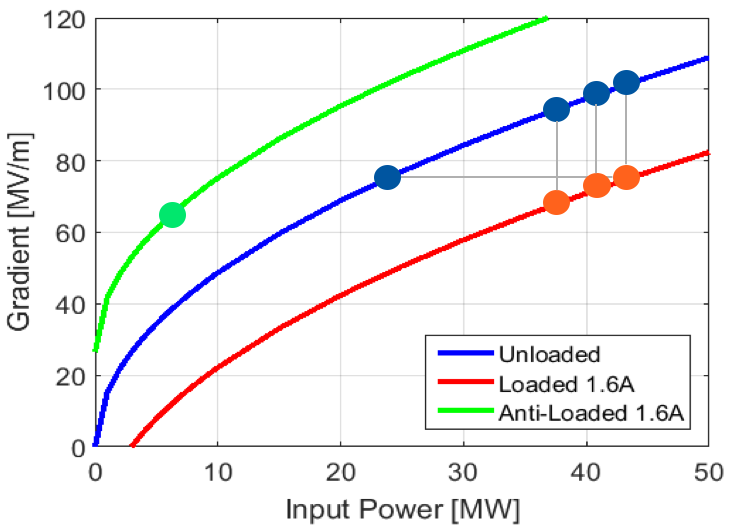
\includegraphics[scale=0.7]{pictures/grad_vs_inPow.png}
\caption{Average gradient as function of the input power in different running conditions. See text for details on the measurement points. }
\label{g_IP}
\end{figure}



\begin{table}
  \centering
    \begin{tabular}{ c l }
    \hline
    \hline
    Run type		&	Input power (MW)		\\
    \hline
    unloaded 		&	43.3, 41, 38 and 24.6	\\
    loaded			&	43.3, 41 and 38			\\
    anti-loaded		&	6.5					\\
    \hline
    \hline
    \end{tabular}
\caption{Input power levels of measurements of 2016 measurement campaign.}
\label{run_pwr}
\end{table}

The measurements at different input power level have not been taken in a precise order, though it has been tried to have as long as possible measurement periods at the same input power. 
The choice was complicated by the fact that the Xbox was not able to provide the maximum RF power level during the full year, mainly because of operational issues, like breakdowns in the pulse compressor and in the waveguide network to the structure, and pulse compressor detuning.


\subsubsection{Comparison of loaded and unloaded runs at same average gradient}

For the CLIC test purpose,  carrying out a measurement at 100 MV/m average gradient comparing loaded and unloaded runs would be the most interesting measurement possible. In order to perform it, the input power has to be raised from 43.3 MW in the unloaded case to 61.3 MW in the loaded case.

Unfortunately, it was clear from the beginning that reaching 61.3 MW of input power was not possible because the waveguides that deliver the power from the pulse compressor to the structure under test had excessive breakdowns for such a high power flux.

Because of this limitation, the choice was limited to perform measurements at the same input power and compare the results, or back off to much lower input power. 

During a period of technical problems, data has been collected for an unloaded measurement at 24.6 MW of input power, which results in a 76 MV/m average accelerating gradient. These can be compared with the the loaded case when running at 43.3 MW of input power, corresponding to an average gradient of 72~MV/m. 

Unfortunately, with a such low input power, the breakdown rate is very low, and after 4 days of measurements zero breakdowns were collected. Therefore it is only possible to set an upper limit to the breakdown rate in these running conditions. Table \ref{comp_avg75} shows the results of the compared running conditions


\begin{table}[h]
  \centering
    \begin{tabular}{ l c c c }
    \hline
    \hline
    Run type							&		Peak(average) gradient  			& BDR ($10^{-5}$ BD pulse$^{-1}$)	\\
    \hline
    Unloaded	@24.6 MW 				&		77 (76) MV/m				&	$< (7.7 \pm 7.7) \, 10^{-3} $ 			\\
    \multirow{ 2}{*}{Loaded  @43.3 MW} 		&		\multirow{ 2}{*}{98 (72) MV/m} 	& 	max. $2.8^{+0.2} _{-0.5}$    		\\
    									&									&	min. $0.3\pm0.09$	\\
    \hline
    \hline
    \end{tabular}
\caption{Gradient parameters and measured breakdown rates for runs near 75~MV/m average accelerating gradient. In the last measured BDR, the error result symmetric because no missed back-off pulse was registered. }
\label{comp_avg75}
\end{table}

The results in Table \ref{comp_avg75} show a significantly higher breakdown rate in the loaded case, where the average gradient is slightly lower, compared to the unloaded case. This consideration allows to conclude that the breakdown rate is not governed by the average gradient.

Using instead the scaling law in Eq.~\ref{E30} and the peak gradient, it is possible to calculate that the expected ratio between the unloaded and the loaded BDR is $0.8\,10^{-3}$, which is compatible with the data collected. 

In order to reproduce the CLIC operational conditions, it is necessary to repeat the experiment in a setup able to support the high power involved, at an average gradient of 100 MV/m.



\subsubsection{Comparison of loaded and unloaded conditions at same input power}

Except for the measurement presented above, it was not possible to compare loaded and unloaded runs at the same average gradient because of the wide difference in input power required. The measurements carried out during the 2016 campaign focused on comparing runs with and without beam at the same input power.  The input power levels used were 43.3, 41 and 38 MW. 

\subsubsection{Study of the antiloaded runs}

The antiloaded measurements were carried out at 6.5 MW of input power. With this input power and a beam current of 1.6 A, the field at the downstream end of the structure reaches the level of the maximum field of the unloaded tests (see Fig.~\ref{3grad}). The results were indeed interesting and will be shown later in the section~\ref{sec:results}. 




\subsection[Beam pulse parameters]{Beam pulse parameters}

As mentioned in the motivation of the experiment, the goal is to understand the effect of the beam on the breakdown rate. The beam parameters have been therefore selected in order to enhance the effect of the beam, rather than trying to simulate the CLIC operation. 

This materialises in:
\begin{itemize}
\item Higher beam current than CLIC: 1.6 A instead of 1.2 A.
\item Longer beam pulse: the beam is present for 250 ns during the whole compressed RF pulse,  while in CLIC will be present at the flat-top of the pulse only. This also keeps the transmitted power level flat.
\end{itemize}
The operation with beam is clearly visible  in the RF signals, as shown in Fig.~\ref{RF_load}. During the loaded operation it can be observed that the transmitted power falls close to zero, because of the energy transferred to the beam. The opposite behaviour can be noted in the antiloaded case, where the input power is much lower than the transmitted. In this case the difference in energy is provided by the beam, that gets slowed down because of the decelerating phase of the RF. 

\begin{figure}[h]
\centering
  \subfigure[Loaded operation]
   {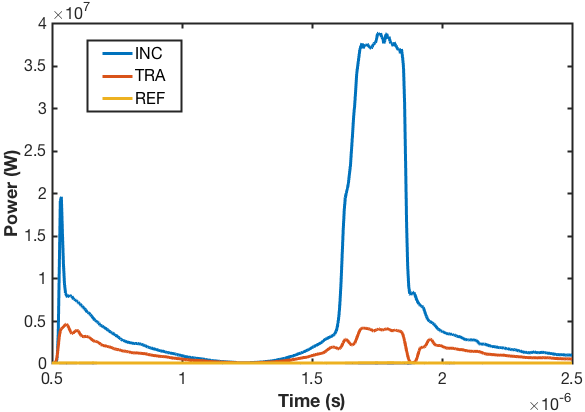
\includegraphics[scale=0.33]{pictures/LoadedPulse.png}}
  \subfigure[Antiloaded operation]
   {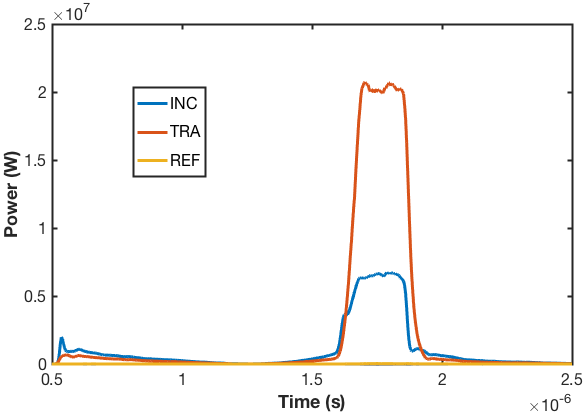
\includegraphics[scale=0.33]{pictures/AntiloadedPulse.png}}
\caption{Comparison of the RF signals during the loaded and antiloaded operation.}
 \label{RF_load}
 \end{figure}


\section[Breakdown rate measurement results]{Breakdown rate measurement results}

The breakdown rate has been calculated for every run, as described in section \ref{sec:BDR}; it is reported in Fig.~\ref{BDR_history} as a function of time. 

A fluctuation of the breakdown rate is appreciable. Considering separately unloaded or loaded runs data at the same input power, the excursion of the fluctuations is about one order of magnitude. Part of this variation could result from an ongoing conditioning of the structure, which might not have reached yet full conditioning.

An unexpected behaviour is observed in July and August, when the BDR is larger at an input power of 38 MW. It is possible that the antiloaded runs between June and July (plotted in green) have some effect on the overall BDR of the following runs. A similar variation of the breakdown rate is observed whenever the input power is changed.

In general, breakdown rate measurements need stable running conditions, and a fluctuation of the BDR is appreciable also in the unloaded tests in the other experiments \cite{Degiovanni:1742280}. Normal measuring times involve measuring periods of the order of weeks. In this experiment, the average stable running time was alternatively four days without beam and 2 days with beam (up to two half-days per week are normally lost in operation and down-time). It is not possible to estimate the impact of this on the breakdown rate. Considering that when changing the input power, the BDR seems to increase, it is reasonable to assume that the accelerating cavity is a system that needs some settling time to stabilise. A similar process could take place when switching from operation with beam to without and vice versa. The reason is that even if the input power remains the same, the field inside is different and the structure needs time to settle. 

A new insight on the effect of the input power variation will be given in the near future from the DC test stand at CERN, that has the possibility to acquire data much faster than any other RF-based experiment \cite{Walter:PC}.

To investigate these effects in the same conditions, it is necessary to repeat the experiment with longer run times. This requires several weeks of dedicated beam time for the loaded runs, that the CTF3 was not able to provide because of the wide experimental program.

\begin{landscape}

\begin{figure}[p]
\centering 
\includegraphics[scale=0.61]{pictures/bdr_hist_2.png}
\caption{History plot of the measured breakdown rate for various measurement conditions.}
\label{BDR_history}
\end{figure}
 
\end{landscape}

One can anyway study the variation of the breakdown rate at the same input power during stable running periods. Figure \ref{BDR_3sectors} shows the detail of three running periods at constant input power. Data show that, at the same input power, the breakdown rate is up to an order of magnitude lower in the loaded case. 

\begin{figure}[h]
\centering 
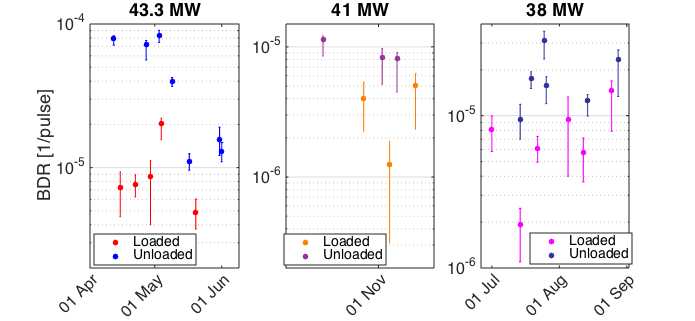
\includegraphics[scale=0.5]{pictures/BDR_zooms.png}
\caption{Comparison of the breakdown rate at different input power in three periods of stable running  at constant input power.}
\label{BDR_3sectors}
\end{figure}

This behaviour can be ascribed to the different field profile in the loaded and unloaded case. In fact, the peak gradient is 5\% lower in the loaded case compared to the unloaded. According to the scaling law in Eq.~\ref{E30}, this difference induces a breakdown rate 3.87 times higher in the unloaded case. Taking into account this factor, the BDR in the loaded and unloaded cases oscillates around the same values. The parameters sustaining this reasoning are reported in Table~\ref{param_var_p}.  These considerations show the data in Fig.~\ref{BDR_3sectors} under a new light: the beam presence itself is not reducing the breakdown rate, but is rather inducing a reduction of the BDR because of the modification of the internal field profile.

\begin{table}[h]
  \centering
    \begin{tabular}{ c c c c }
    \hline
    \hline
    Input power 		&		$E^\text{unloaded} _\text{peak}$ (MV/m)		& 	$E^\text{loaded} _\text{peak}$ (MV/m)		&	$\left ( E^\text{unloaded} _\text{peak} / E^\text{loaded} _\text{peak} \right )^{30}$	\\
    \hline
    43.3 MW		&		102.6 								&	98.1									&	3.87		\\
    41 MW			&		99.9 									&	95.5									&	3.87		\\
    38 MW			&		96.1 									&	91.9									&	3.87		\\
    \hline
    \hline
    \end{tabular}
\caption{Gradient parameters for runs with and without beam at the same input power. E$_\text{peak}$ is the peak accelerating gradient. The loaded data are calculated using a current of 1.6 A.}
\label{param_var_p}
\end{table}

It has to be noted that there are two exceptions to the behaviour outlined above: an unloaded run at 43.3MW input power at the end of March (plotted in blue in Fig.~\ref{BDR_history}), and the last loaded runs of the year at 38 MW input power (see dedicated plot in Fig.~\ref{BD_prob_last_raise}). 

In the first case, it is not clear why the BDR was that low, it represents a clear anomaly considering the general trend of the precedent runs. It also has to be pointed out that the run is shorter than the others, so the statistical fluctuations might play a role.

Regarding the second case, the BDR of the loaded and unloaded runs seems to converge at the end of the year. In addition, the last loaded run presents a higher BDR than the previous and following unloaded runs. The result may be ascribed to a statistical fluctuation, but  it was impossible to verify this further because of the stop of the experiments at the end of the year.

\begin{figure}[h]
\centering 
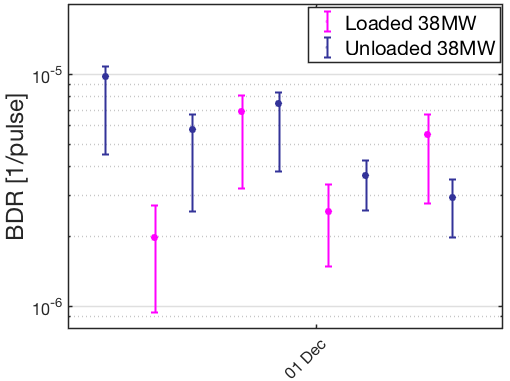
\includegraphics[scale=0.55]{pictures/BDR_last_part_year.png}
\caption{Measured breakdown rate at the end of the year.}
\label{BD_prob_last_raise}
\end{figure}





\section[Breakdown distribution]{Breakdown distribution}

\subsection[A model for the breakdown distribution]{A model for the breakdown distribution}

Unloaded experiments exhibit an approximately linear distribution of the breakdowns with the field in the accelerating structure. In addition, it is known that the overall structure breakdown rate follows the scaling law in Eq.~\ref{E30}, but this has been derived from the data available from unloaded tests as well. These considerations urge one to try to understand if these results are still valid when running with the beam inside the accelerating cavity.

Considering any cell as a substructure, it is reasonable to suppose that cells with a higher accelerating field will be more likely to experience breakdowns than cells with a lower field. According to this reasoning and following the Eq.~\ref{E30}, the breakdown probability per cell is given by
\begin{equation}
\text{BD probability} =\frac{   \left ( \frac{E_\text{cell}}{E_\text{max}} \right )^{30} }{ \sum \left( \frac{E_\text{cell}}{E_\text{max}} \right )^{30}   } 
\label{scal_eq_prob}
\end{equation}
where E$_\text{cell}$ is the maximum surface electric field of the cell and E$_\text{max}$ is the maximum surface electric field of all the cells. 

The choice of using the surface electric field instead of the accelerating gradient comes from the physics of the breakdown process \cite{Walter:PC}. Anyway the shape of the gradient profile and of the surface electric field along the structure differ only slightly. The field of the coupling cells is assumed to be identical to the adjacent cells. This comes from geometrical considerations, and could be eventually derived from simulations \cite{Alexej:PC}.

The breakdown probability vs cell number is shown in Fig.~\ref{BD_prob}. The expectation is to have a flatter distribution compared to the others in the unloaded case, with an accumulation of the number of breakdowns in the first part of the structure for the loaded case and at the end of the structure for the antiloaded case.


\begin{figure}[h]
\centering 
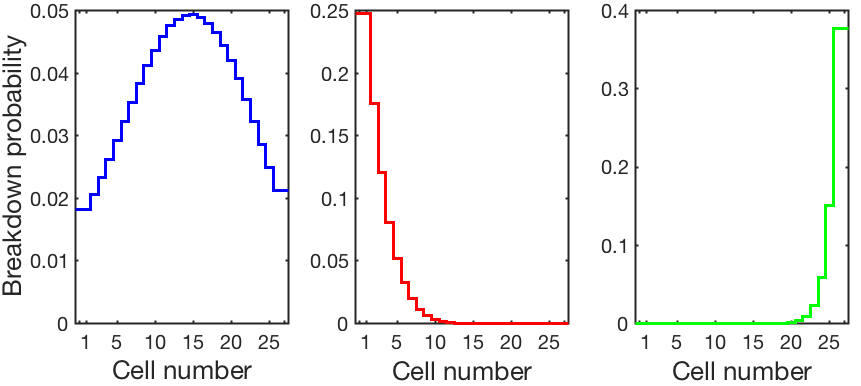
\includegraphics[scale=0.45]{pictures/BD_probability_2.png}
\caption{Breakdown probability according to the model in different running conditions: unloaded (left), loaded (center), antiloaded (right). The different scale has to be noted: while the breakdown probability oscillates between the 1.8\% and 5\% in the unloaded case, when the beam is present the difference is much bigger.}
\label{BD_prob}
\end{figure}


\subsection[Measurement results]{Measurement results}
\label{sec:results}

The breakdown distributions, for data at the same input power are shown in Fig.~\ref{BD_distro}. Both a linear scaling with the surface field and the scaling proposed in the previous section are plotted together with data.

In the centre of the structure there is a more active part, where a large number of breakdowns are happening. This active region is present both in the unloaded and loaded runs, and could be provoked by: 
\begin{enumerate}
\item the development of an \textit{hot cell}, which is a concentrated accumulation of breakdowns in a small area, usually an iris. This causes surface damage, that enhance field emission and breakdown clustering in the vicinity of the damaged area~\cite{Wang:2008ap}. The development of an hotcell happened in the past, and required the substitution of the structure.
\item slight surface damage of the central cells, where for some reason the surface is rougher and provokes more breakdowns. 
\end{enumerate}

\begin{landscape}

\begin{figure}[p]
\centering 
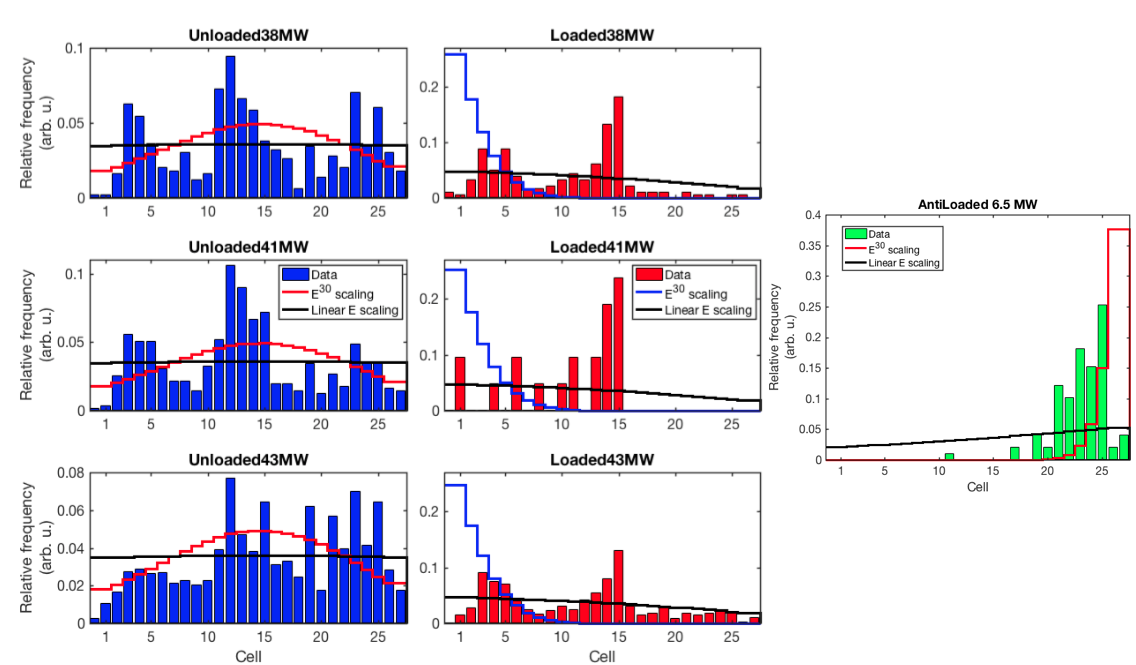
\includegraphics[scale=0.53]{pictures/distro_all.png}
\caption{Measured breakdown distribution in the accelerating cavity under test in different running conditions. Superimposed, the scaling of Eq.~\ref{scal_eq_prob} is plotted in red and a linear scaling with the surface field is plotted in black.}
\label{BD_distro}
\end{figure}
 
\end{landscape}



Fortunately, there is no sign of the development of an hotcell. Figure~\ref{BD_3d} shows that although a more active region in the centre developed after the antiloaded runs in June 2016, it was gradually reconditioned during the following part of the year. 

Additional hints will come from the post-mortem analysis of the structure, that will be cut and examined with various microscopy techniques. This analysis will take place later in 2017. In any case, the second option looks the most probable. 

If one ignores this central region, the breakdown distribution is compatible with a constant distribution during runs without beam. It is also compatible with the hypothesis of accumulation of the breakdowns in  the first part of the structure during the loaded runs and at the end during the antiloaded runs, in the regions with the higher field.

Both the linear and the power law breakdown scaling do not match the measured distribution well. Even ignoring the central active zone, it is not clear which law rules the distribution of the breakdowns in the cells. Collecting more data is necessary for this purpose.

\begin{figure}[h]
\centering 
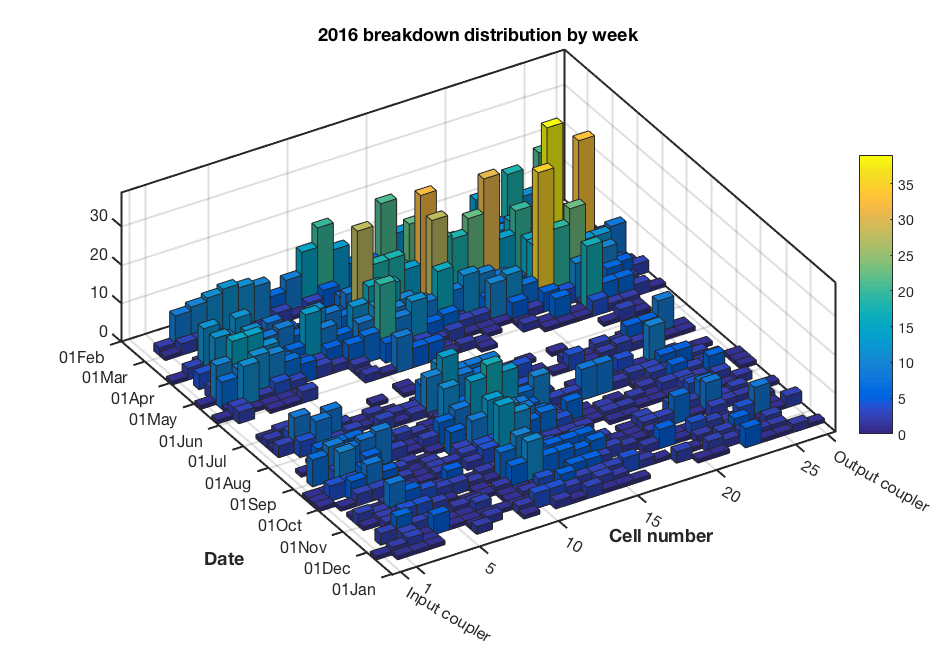
\includegraphics[scale=0.4]{pictures/week_distr_3D.png}
\caption{Breakdown number per cell per week. }
\label{BD_3d}
\end{figure}








\newpage
\section[Beam induced RF power]{Beam induced RF power}

It is interesting to observe the effect of the beam on the RF signals after a breakdown. Figure \ref{BI_rf_fig}  shows two examples of RF signals. Three phases are clearly visible in the transmitted power signal: 
\begin{enumerate}
\item the power falls after the breakdown because of the reflection of the RF caused by the plasma.
\item the beam keeps passing through the plasma. The part of the cavity after the breakdown is not filled anymore by the incident RF, and the beam starts to produce power getting decelerated because passing through an empty cavity. This process has a short duration and results in a spike in the power produced. 
\item the power production stabilises with the establishment of a plateau in the transmitted power profile.
\end{enumerate}
At the moment there is no satisfactory theory that explains the behaviour of the RF power production in the cavity after the breakdown. Hence it is not clear which process is provoking the observed power spike.

Two different examples are presented in the figure. The spike is visible on the right, but the plateau does not have time to develop because of the end of the beam pulse. On the left the full development of the process is appreciable.

\begin{figure}[h]
\centering
  \subfigure[Breakdown happening early in the pulse]
   {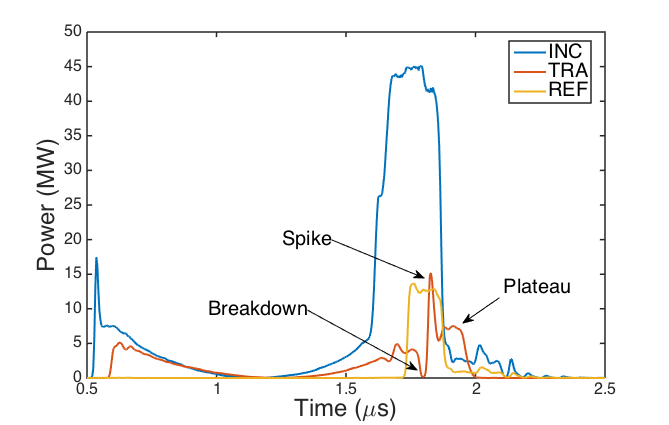
\includegraphics[scale=0.33]{pictures/BI_rf.png}}
   \hspace{2mm}
  \subfigure[Breakdown happening late in the pulse]
   {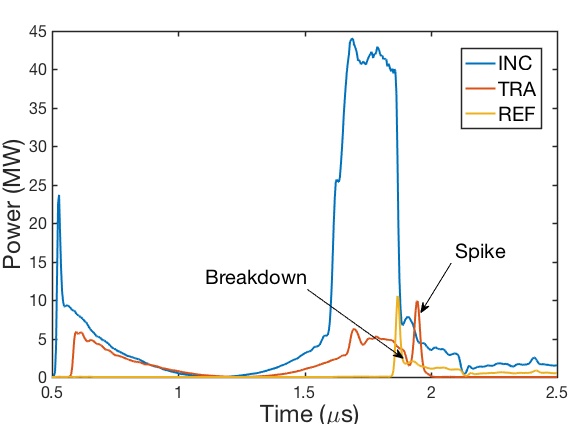
\includegraphics[scale=0.33]{pictures/BI_rf_2.png}}
\caption{Two examples of RF signals for a breakdown event earlier and later in the pulse. In both cases the spike provoked by the beam-induced RF production is visible. In the early case (a) it is possible to see the development of the plateau induced by the stabilisation of the power production up to the end of the beam pulse. In the late case (b) the beam pulse duration is not sufficient to allow the development of a stable condition.}
 \label{BI_rf_fig}
 \end{figure}

\newpage
\section{Conclusions}

The experiment described in this work offers a first glimpse on the beam effect on the breakdown rate in a normal-conducting travelling-wave accelerating structure.

During the 2016 measurement campaign, the expertise to realise breakdown experiments with the beam has been gained. The experiment was carried out with a longer beam pulse and with higher current than the CLIC Main Beam parameters to enhance the effect of the beam on the BDR.

A fundamental result is that the breakdown probability is ruled by the peak accelerating gradient, and not by the average accelerating gradient.

This work showed that the breakdown rate is in general lower during experiments with the beam, performed with the same input power. This difference can be ascribed to the internal field profile modification induced by the beam presence, which results in a lower peak accelerating gradient.

The distribution of the breakdowns in the accelerating cavity follows the field distribution, resulting in the majority of the breakdowns happening in the front part of the structure when accelerating the beam and in the last part when decelerating. Unfortunately, the development of an active zone in the centre of the structure makes it impossible to find the scaling law for the breakdown distribution. 

A different migration dynamics of the breakdowns have been detected during the loaded and antiloaded runs. This could be explained by the modified field profile induced by the loading of the cavity with the beam.

Further investigations in this field require to repeat the experiment in more stable conditions, with measurements of long duration (weeks). This last request translates into long beam times that the tight scientific program of the CTF3 was not able to provide. Missing this condition, it is not possible to understand if the continuous switching between different running conditions impacts on the fluctuation of the breakdown rate. Anyway it is reasonable to expect that this causes a higher fluctuation of the breakdown rate than the one achievable running in stable conditions. 

The experiment can be considered successful, because of the amount of information that have been collected, even with a limited and not continuous beam time in a non-dedicated experiment.



\section[Further developments]{Further developments}

The experience gained from this work allows one to suggest some modifications to the setup, starting by the newer Xboxes:
\begin{itemize}
\item The substitution of the TWT with a solid state amplifier will avoid the presence of spikes. The new amplifier has been installed in XBOX1 at the beginning of 2017.
\item Switching the pulse compressor from SLED-I to SLED-II type (as is in Xbox2), and placing the Xbox closer to the structure under test would solve the detuning problem (since the attenuation of the waveguides is lower and the power requested from the pulse compressor as well).
\item The missing back-off in power has to be investigated and solved. Probably the performance of the interlock system program running on the FPGA could be improved by writing the related code in a hardware description language instead of LabVIEW.
\item The sampling rate of the log detectors could be improved up to 1 GSa/s using the same acquisition system used for the IQ detectors.
\end{itemize}

On the physics side, pursuing the experiments in a dedicated facility would be the optimal solution. As a general guideline, alternating several weeks of experiments with beam with weeks of unloaded experiments could be a good programme. This should allow one to get more meaningful results and compare with the unloaded results of the Xboxes, where the normal experiment time is weeks.

Finally, before the implementation of CLIC, an experiment operating in the CLIC conditions would be very interesting. In particular, the comparison of the loaded and unloaded operation of the cavity at 100 MV/m average gradient would be extremely interesting.